\documentclass{article}
\usepackage{amsmath}
\usepackage{graphicx}
\usepackage{booktabs}
\usepackage{verbatim}
\usepackage{pdfpages}
\usepackage{pgfplots}
\usepackage{textcomp}
\usepackage{algorithm}
\usepackage{algpseudocode}
\usepackage{pifont}
\usepackage{backref}


\begin{document}

\tableofcontents
\listoffigures
\listoftables
\newpage
\pagenumbering{arabic}
\section{First One}
\begin{equation}
  f(x) = x^2
\end{equation}

\subsection{Second One}
\begin{equation}
  f(x) = x^2
\end{equation}
\newpage
\section{Third One}
\begin{equation*}
  f(x) = x^2
\end{equation*}
\newpage
\section{Fourth One}
\begin{equation*}
  f(x) = x^2
\end{equation*}
\subsection{Fifth One}

\begin{equation*}
  f(x) = x^2
\end{equation*}
This formula $f(x) = x^2$ is an example.


\begin{equation*}
  1 + 2 = 3 
\end{equation*}

\begin{equation*}
  1 = 3 - 2
\end{equation*}

\begin{align*}
 F(x) &= \sum^{UDB.size()}_{i=0} [ \frac{1}{3}x^3 ]
\end{align*}

%\begin{figure}
%  
\includegraphics[width=\linewidth]{boat.jpg}
%  \caption{A boat.}
%  \label{fig:boat1}
%\end{figure}
%Figure \ref{fig:boat1} shows a boat.

\newpage
\section{Table Section}
\subsection{First Table}
\begin{table}[h!]
  \begin{center}
    \caption{Caption for the table.}
    \label{tab:table1}
    \begin{tabular}{l|c||r}
      1 & 2 & 3\\
      \hline
      a & b & c\\
    \end{tabular}
  \end{center}
\end{table}

\subsection{Second Table}
\begin{table}[h!]
  \begin{center}
    \caption{Caption for the table.}
    \label{tab:table2}
    \begin{tabular}{ccc}
      \toprule
      Some & actual & content\\
      \midrule
      prettifies & the & content\\
      as & well & as\\
      using & the & booktabs package\\
      \bottomrule
    \end{tabular}
  \end{center}
\end{table}
\newpage

\section{Algorithm}

\begin{algorithm}
\caption{CH election algorithm}
\label{CHalgorithm}
\begin{algorithmic}[1]
\Procedure{CH\textendash Election} {}
\For{each node $i$ \Pisymbol{psy}{206} $N$ }
\\Broadcast HELLO message to its neighbor
\\let $k$ \Pisymbol{psy}{206} $N1$ ($i$) U {$i$} be s.t
\\QOS($k$) = max {QOS($j$) \textbar $j$ \Pisymbol{psy}{206} $N1$($i$)  U $i$}
\\ MPRSet($i$) = $k$
\EndFor
\EndProcedure
\end{algorithmic}
\end{algorithm}
\pagebreak
\newpage
\section{GRAPH PDF INSERTION}

\includepdf[pages={1}]{graph.pdf}
\newpage
\section{Diagram}

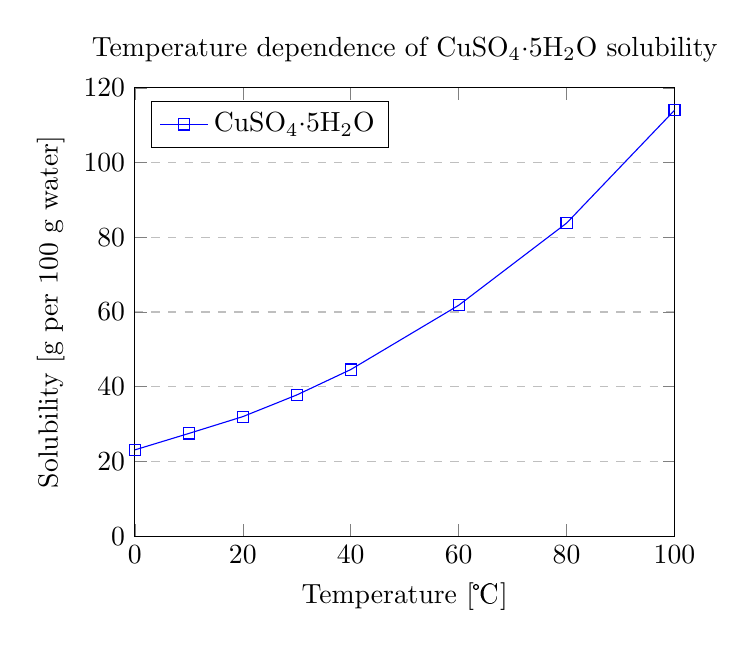
\begin{tikzpicture}
\begin{axis}[
    title={Temperature dependence of CuSO$_4\cdot$5H$_2$O solubility},
    xlabel={Temperature [\textcelsius]},
    ylabel={Solubility [g per 100 g water]},
    xmin=0, xmax=100,
    ymin=0, ymax=120,
    xtick={0,20,40,60,80,100},
    ytick={0,20,40,60,80,100,120},
    legend pos=north west,
    ymajorgrids=true,
    grid style=dashed,
]
 
\addplot[
    color=blue,
    mark=square,
    ]
    coordinates {
    (0,23.1)(10,27.5)(20,32)(30,37.8)(40,44.6)(60,61.8)(80,83.8)(100,114)
    };
    \legend{CuSO$_4\cdot$5H$_2$O}
 
 \end{axis}
\end{tikzpicture}

\end{document}
